\subsubsection{Vecindario}
    \label{sec:Vecindario}
    Un vecindario es un conjunto de celdas que se toman en cuenta para la actualizaci\'on de una celda. Como vimos con anterioridad
        en los aut\'omatas celulares de una dimensi\'on, el vecindario de una celda es la celda y sus dos vecinos, pero en los aut\'omatas
        celulares de dos dimensiones el vecindario de una celda puede ser de cualquier tama\~no, siempre y cuando sea sim\'etrico, es decir,
        que la celda se encuentre en el centro del vecindario. En la figura \ref{fig:mooreN} se puede ver un ejemplo de un vecindario
        de una celda. E incluso en los aut\'omatas celulares de dos dimensiones se pueden tener vecindarios de diferentes formas, como se
        es com\'un verlos en forma cuadrada y en forma hexagonal.
    \vskip 0.5cm
    A su vez los vecindarios m\'as usados son los siguientes: 
    \begin{itemize}
        \item 
            \begin{minipage}
                {0.5\textwidth}
                \textbf{Vecindario de Moore} En este caso el vecindario de una celda es la celda y sus ocho vecinos.
            \end{minipage}
            \begin{minipage}{0.5\textwidth}
                \centering
                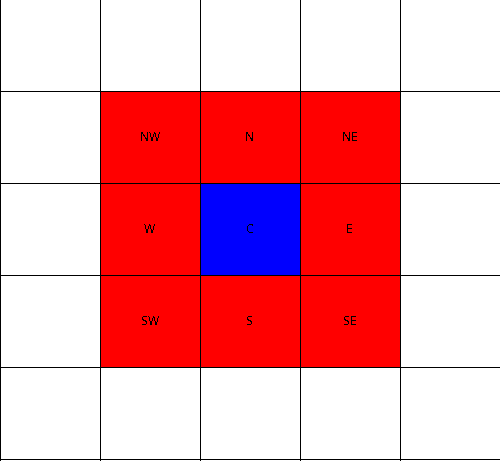
\includegraphics[width=0.5\textwidth]{./images/marco_teorico/automatas_celulares/mooreN.png}
                \captionof{figure}{Vecindario de Moore}
                \label{fig:mooreN}
            \end{minipage}
        \item
            \begin{minipage}
                {0.5\textwidth}
                \textbf{Vecindario de von Neumann} En este caso el vecindario de una celda es la celda y sus cuatro vecinos.
            \end{minipage}
            \begin{minipage}
                {0.5\textwidth}
                \centering
                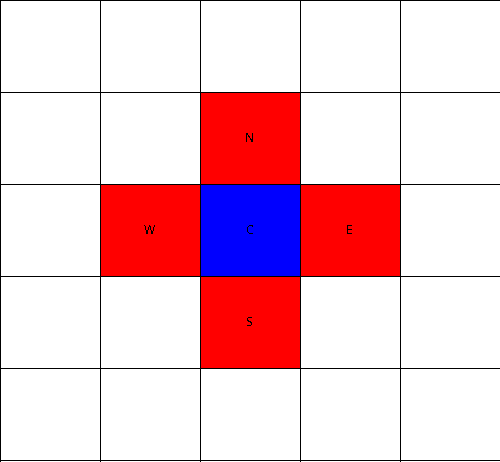
\includegraphics[width=0.5\textwidth]{./images/marco_teorico/automatas_celulares/vonN.png}
                \captionof{figure}{Vecindario de von Neumann}
                \label{fig:vonN}
            \end{minipage}
        \item
            \begin{minipage}
                {0.5\textwidth}
                \textbf{Vecindario de Moore extendido} En este caso el vecindario de una celda es la celda y sus veinticuatro vecinos.
            \end{minipage}
            \begin{minipage}
                {0.5\textwidth}
                \centering
                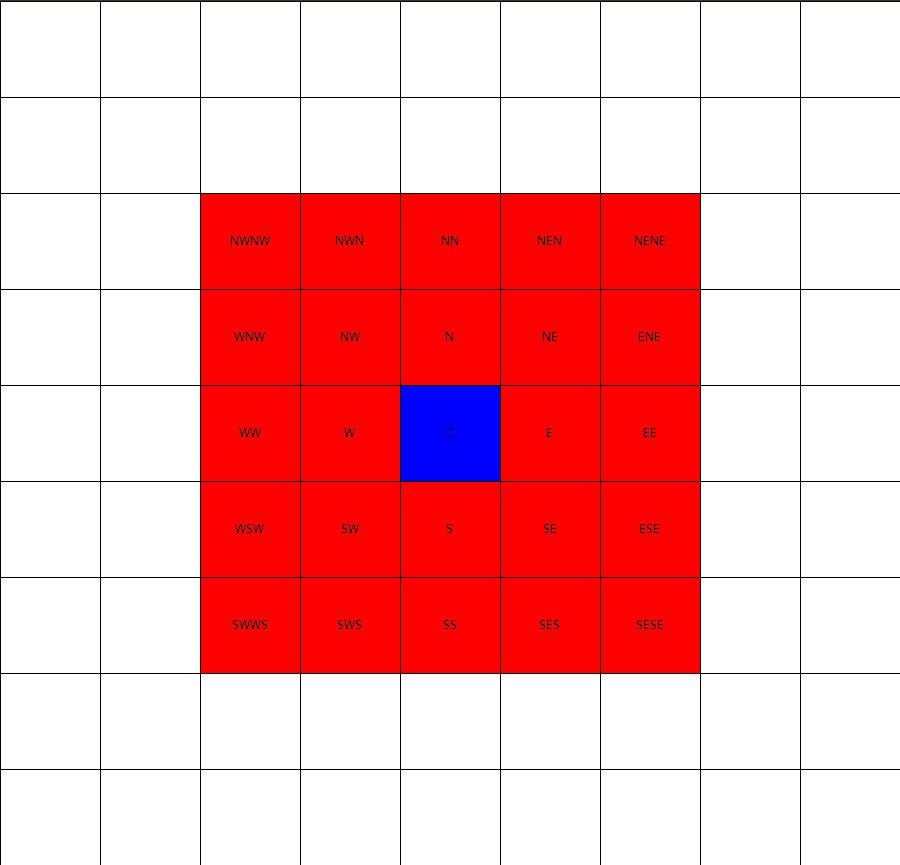
\includegraphics[width=0.5\textwidth]{./images/marco_teorico/automatas_celulares/mooreNeX.jpg}
                \captionof{figure}{Vecindario de Moore extendido}
                \label{fig:mooreNeX}
            \end{minipage}
        \item 
            \begin{minipage}
                {0.5\textwidth}
                \textbf{Vecindario de von Neumann extendido} En este caso el vecindario de una celda es la celda y sus doce vecinos.
            \end{minipage}
            \begin{minipage}
                {0.5\textwidth}
                \centering
                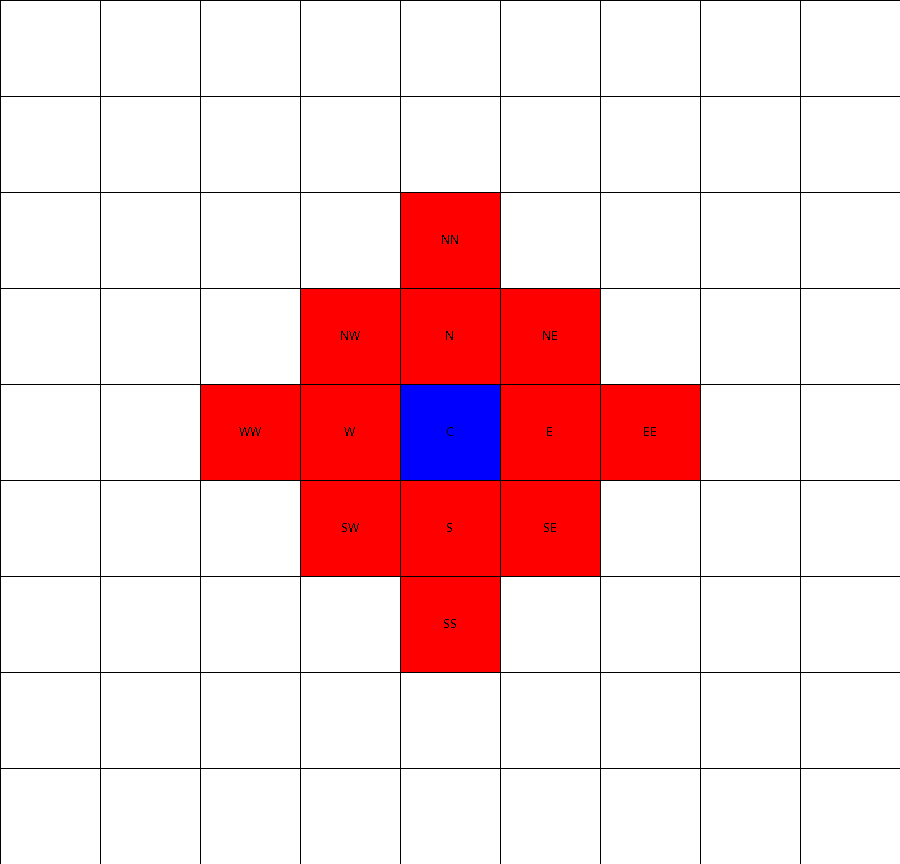
\includegraphics[width=0.5\textwidth]{./images/marco_teorico/automatas_celulares/vonNeX.png}
                \captionof{figure}{Vecindario de von Neumann extendido}
                \label{fig:vonNeX}
            \end{minipage}
        \item
            \begin{minipage}
                {0.5\textwidth}
                \textbf{Vecindario de hexagonal} En este caso el vecindario de una celda es la celda y sus seis vecinos.
            \end{minipage}
            \begin{minipage}
                {0.5\textwidth}
                \centering
                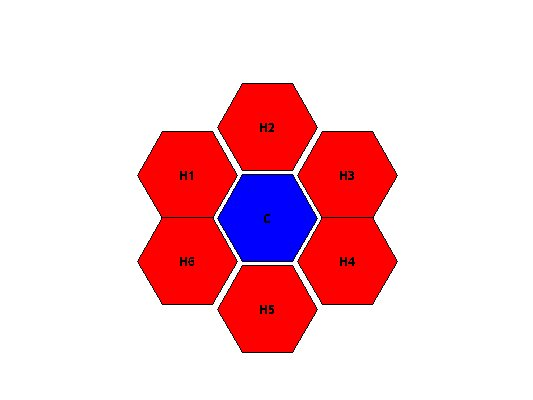
\includegraphics[width=0.5\textwidth]{./images/marco_teorico/automatas_celulares/hexN.jpg}
                \captionof{figure}{Vecindario de hexagonal}
                \label{fig:hexN}
            \end{minipage}
    \end{itemize}
    \vskip 0.5cm
    Una vez que hemos explicado eso podemos pasar a definir formalmente los aut\'omatas celulares.
    \vskip 0.5cm